\chapter{Introduction}\label{ch:intro}

\section{Dual-Settlement Nodal Electricity Markets}\label{sec:dual-settlement-nodal-electricity-markets}

The increasing integration of renewable energy sources into the electrical grid has led to heightened volatility and
uncertainty in electricity prices.
This presents a major challenge for electricity market participants, who must be able
to accurately forecast electricity prices in order to make informed investment and trading decisions.
To address this challenge, the application of machine learning, and in particular deep generative models, to
day-ahead electricity price forecasting has become a topic of significant interest.

The North American electrical grid, sometimes regarded as the ``world's largest machine'', is a feat of modern
engineering and operations that provides a critical resource for over 400 million of individuals.
While the planning, construction, and maintenance of the physical infrastructure a clearly non-trivial tasks,
post-completion the continuous and efficient operation of grid resources poses perhaps an even greater challenge.
In order to keep generation and demand need to be synchronized, a grid operator must dispatch the least-cost optimal
generators at the perfect time.
Furthermore, the matching must be done continuously despite uncertainty in the load, weather, generation,
grid topology, fuel prices, etc., lest there be a catastrophic failure in overall grid operations~\cite{ercotfail}.

The early grid worked with local, vertically integrated utilities that owned all the generation and transmission in
an area.
Due to the small scale of the grids and relative certainty in the generation mix, real time dispatch remained simple
enough such that it could be done manually.
Growth in the size and interconnection of the grid network has exacerbated the nonlinear and often extreme interactions
between components in an alternating-current (AC) network~\cite{grid_sensitivity}.
More recently, increased penetration of renewable energy sources, such as solar and wind generation, coupled
with a lack of suitable storage options has dramatically increased overall uncertainty in grid operations.
One proposed solution to these challenges is the deregulation of the wholesale energy market with the development of
the locational marginal price (LMP) model and competitive bid-based market[CITE].
Roughly two-thirds of U.S. electricity consumers live in a region serviced by such markets, and similar efforts are
actively pursued in European energy markets under the moniker ``energy liberalisation.''

These new, competitive energy markets allow electricity generators to offer their capacity for sale to load-serving
entities, such as utilities and large energy consumers.
These markets are organized by independent system operators (ISOs), which are responsible for ensuring the reliability
of the electrical grid and fair markets for participants.
ISOs offer multiple different markets, typically defined by the time-frame of trades, to allow participants to hedge
against price volatility.
One example is the day-ahead (DA) market, a forward market where electricity is traded on the day prior to delivery.
Generators submit bid-curves stating how much they are able to produce and at what price, and load-serving
entities (LSEs) such as utilities bid their customer's forecasted demand into the markets.
Speculators play an additional role in assuming the excess risk that is unpalatable to LSEs and generators.
After the trades are cleared and aggregated, the ISO formulates a locational marginal price (LMP) at locations on the
grid, often referred to as \textit{price nodes}.
The LMP can be decomposed into the \textit{energy price}, \textit{congestion price}, and \textit{loss price} which are
the costs of producing the energy (equal at all nodes), the costs of safely transmitting energy across the grid,
and the energy loss due to physical transmission inefficiencies.
Figure~\ref{fig:contours} captures a subset of LMPs in the Pennsylvania-New Jersey-Maryland (PJM) ISO at various times
of a typical market day.
Observe the near constant LMPs in the early morning hour of the market (top-left) and the significant differences
between nearby prices nodes in the afternoon hours (bottom-left) indicating low-congestion and high-congestion
regimes respectively.

\begin{figure}[htbp]
    \caption[Contour map of PJM DA LMPs at various times on a single market-day ]{
        Nodal day-ahead LMPs and the contours interpolated prices in areas between nodes.
        White circles depict the location of target price nodes in PJM whose prices are reflected in the
        inscribed colors.
        Prices between nodes are interpolated using radial-basis-function kernel interpolation.
    }
    \begin{center}
        \setlength{\fboxsep}{0pt}%
        \setlength{\fboxrule}{1pt}%
%        \fbox{
        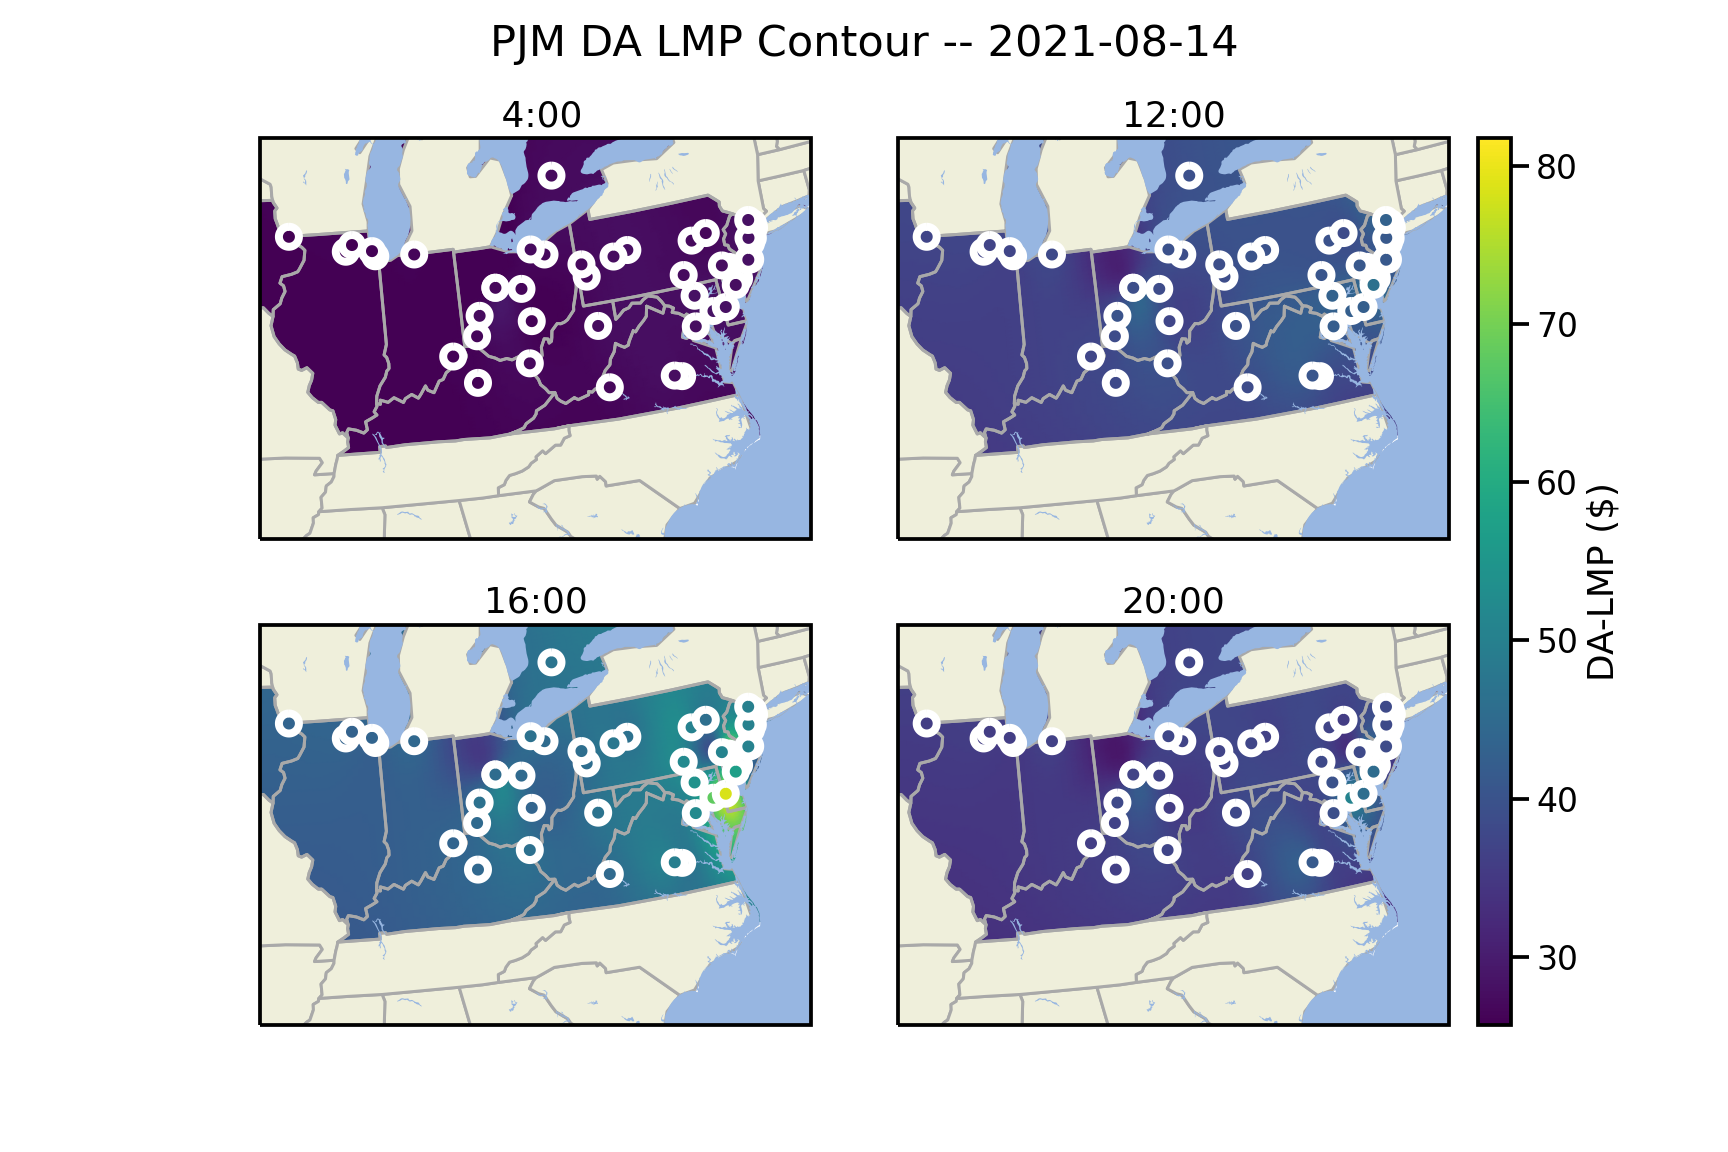
\includegraphics[width=150mm]{figs/pjm_lmp_contour_singlecbar}
%        }
    \end{center}
    \label{fig:contours}
\end{figure}

\section{The Application of Machine Learning to Price Forecasting}\label{sec:the-application-of-machine-learning-to-price-forecasting}

The complicated task of forecasting nodal LMPs play a crucial role in the functioning of DA markets.
Accurate forecasts allow market participants to make informed trading decisions, plan generation and demand schedules,
and manage risk exposure.
Thus poor forecasts can result in reduced market efficiency, realized by wasted generation
resources and high prices.
Factors such as volatile renewable generation, weather patterns, fuel prices, demand uncertainty, and complex
interactions between grid components make it a formidable challenge.
However, recent developments in machine learning, in particular deep learning methods, and access to historical market
data show promise at capturing the complex and dynamic structures essential for accurate forecasts.

\section{Related Work}\label{sec:related-work}

Energy price forecasting literature can be split roughly into three categories: \textit{system pattern} (SP)
methods, statistical and machine learning methods, and deep-learning methods.

The work of Zhou et al.~\cite{5741753} develop the idea of SPs as an exploitation in the structure of the LMP optimization
problem formulation, where predictable market characteristics and associated \textit{system pattern regions} (SPRs), or
continuous neighborhoods of market conditions, represented by polytopes in load space give rise to specific predictable SPs.
Forecasting price action is then reduced to estimating which SPRs future market conditions will map to, and subsequently
retrieving the likely SPs and price action.
To overcome bias in the set of observed market states, a ``probabilistic'' formulation is also presented that can report
upper and lower quantile forecasts along with a mean forecast.
However, the SPR state space suffers from the curse of dimensionality, making analysis of large grids computationally
intractable.
Geng et al.~\cite{7478156} build upon the SPR concept, showing that they can be constructed using data driven
methods, in particular learning SPR classification boundaries with support vector machines.
These data driven SPR techniques are, however, still computationally intractable for anything more than small, synthetic
grid examples.
Radovanovic et al.~\cite{8733097} expand upon a similar idea to SPRs.
Through the use of recent advances in compressed sensing they reconstruct grid topologies allowing downstream inference
and clustering of congestion prices.
Clusters of generation-mix and load forecast are mapped to price clusters allowing for LMP forecasting.
These SPR-like representations makes this method significantly more scalable for inference, however, training
the model incurs a costly step of reconstructing grid topology which can be significant for large grids~\cite{7226869}.

Using traditional statistical methods and machine learning methods, Uniejewski et al.~\cite{en9080621} propose a linear
auto-regressive model using ordinary least squares regression and LASSO automatic feature selection techniques.
This linear model can be modified for quantile regression tasks~\cite{UNIEJEWSKI2021105121} or with advanced
jump-diffusion and timeseries techniques to produce probabilistic forecasts~\cite{MUNIAIN20201193}.
Andrade et al.~\cite{00000} present a methodology for both point and quantile forecasts using robust gradient boosting
trees and linear quantile regression, coupled with post-processing that exploits daily average prices to increase
forecast quality.

Deep-learning methods have recently risen in popularity for energy forecasting, beginning with the work of
Wang et al.~\cite{7744689} who present a stacked de-noising auto-encoder (SDA) neural network with unsupervised
pre-training and supervised fine-tuning regimes to improve forecast accuracy.
Subsequent work by Lago et al.~\cite{LAGO2018386} compare novel deep feed-forward neural network (DNN),
convolution neural network (CNN), and recurrent neural network (RNN) architectures and demonstrate the superiority of
deep-learning methods over traditional statistical methods.
A two stage convolutional long short term memory (CLSTM) neural network to first
forecast generation bid curves to improve second stage LMP point forecasts is proposed in~\cite{9916722}.
Zhang et al.~\cite{9520248} introduce a generative adversarial network (GAN) using a novel 3d tensor structure and
convolutional neural network to learn the spatio-temporal interactions from the tensor representation.
%A caveat of this method is the mapping of historical data
%observations to a 2D-tensor is ambiguous, which means that ``spatial'' interactions learned
%will be sensitive to the layout data in the tensor. Additionally, despite having cabablities
%for probabilistic forecasts by taking multiple samples from the GAN the authors only explore
%the single point forecasts with the model.
Cramer et al.~\cite{48550} develop a normalizing flows model capture the joint probability distribution of multi-hour price
action on a single node and generate probabilistic forecasts for intra-day nodal prices in the German EPEX spot market.

\section{Motivation}\label{sec:motivation}

We motivate the formulation of probabilistic forecasts by first illustrating the drawbacks to both point and interval
forecasts.
Consider a participant who obtains point forecasts.
It is not surprising if they begin to ask questions not only on the accuracy of the forecast but also on what is not
included in the forecast, ``What is the probability the true price will be above/below my forecast?
How likely is my forecast to be \$10 under/over the true price?
What about \$100 over/under?''
The implied financial risk of accepting a point forecast at face value an be astronomical, but without an accurate and
informative measure of uncertainty the options to determine that risk are limited and rely on further assumptions which
likely do not hold in reality.

While interval forecasts offer some benefit over point forecasts, they continue to discard information that
that could be useful for decision-making.
For instance, while a 95\% confidence interval forecast surrounding a point forecast provides greater insight on the
likelihood of facing financial ruin than a point forecast, information on the distribution inside the confidence
interval such as skewness, multi-modality, or tail behavior is still unknown.

Such needs simply cannot be fulfilled by point and interval forecasts despite the accuracy and sophisticated means of
obtaining the forecasts.
However, recent advances in deep neural network based generative models, in particular \textit{normalizing flows}, allow
for both estimating the likelihood of events and efficient sampling of high-dimensional conditional probability densities,
enabling simple yet flexible powerful Monte Carlo estimation of key quantities of interest needed to make informed
financial decisions in energy markets.

The rest of this work is structured as follows.
In Chapter~\ref{ch:background} we outline the key mathematical background required to formulate probabilistic forecasts
using recent advances in deep generative modeling.
In Chapter~\ref{ch:methodology} we define our proposed methodology for characterizing probability density estimators
and generating probabilistic forecasts.
In Chapter~\ref{ch:experiments} we investigate techniques to improve forecasting skill in day-ahead energy markets and
compare our proposed methods against open-benchmarks in energy price forecasting literature and commercial price
forecasting tools.
Finally, in Chapter~\ref{ch:conclusion} we summarize our key findings and lay out key future research paths to improve
model results, robustness, interpretability, and generalizability.
